\chapter{Notational Conventions and Preliminaries}
\label{ch-conventions}
This book is a sequel to
my book entitled \qt{Bayesuvius}
(see Ref.\cite{bayesuvius}). 
For consistency, 
I have tried to follow in this book the 
same notational conventions
used in the prior book.
If any notation is not defined in this book,
check in the prior book. It might be
defined there.  

\section{Set notation}

Definitions

$|S|$ = the number of elements in a set $S$.
(known as its {\bf order, size, length, cardinality})

$\ZZ$ = integers

$\ZZ_{>0}$ = positive integers

$\ZZ_{[a,b]} = a, a+1, \ldots, b$
for some integers $a, b$ such that $a\leq b$

$\RR$ = reals

$\QQ$= rationals

$\CC$ = complex numbers

$\CC^{n\times m}$ = $n\times m$ matrices of complex numbers

\section{Commutator and Anti-commutator}
Let

{\bf commutator of $A$ and $B$}
\beq
[A, B] = AB-BA
\eeq

{\bf Anti-commutator of $A$ and $B$}
\beq
[A, B]_+ = AB+BA
\eeq

\section{Equivalence Relation}
An {\bf equivalence relation} $R$ on a set $X$ is a subset of $X\times X$
that satisfies the 3 axioms given below. One writes $a\sim b$ or $aRb$ instead of $(a,b)\in R$. For all $a,b,c\in X$, $R$
must satisfy:

\begin{enumerate}
\item reflexive: $a\sim a$ 
\item symmetric: if $a\sim b$ then $b\sim a$
\item transitive: if $a\sim b$ and $b\sim c$ then  $a\sim c$.

\end{enumerate}

An {\bf equivalence class} of $R$ is a set 
$C(a)=\{x\sim a\mid x\in X\}$.
All possible equivalence classes of $R$ 
constitute a disjoint partition of $X$:

\beq
X= \bigcup_{a\in X} C(a)
\eeq

\beq
C(a) \cap C(b)=\emptyset \text{ iff }  C(a) \neq C(b)
\eeq

\section{Direct Sum and Direct Product of Matrices}

For any square matrices $A$, $B$, $C$ (not necessarily of the same dimension)
\beq
A\oplus B\oplus C = \begin{pmatrix}
A&0&0
\\0&B&0
\\
0&0&C
\end{pmatrix}
\eeq
If $A_i$ for $i=1,2, \ldots, n$ are square matrices, $A_1\oplus A_2 \oplus \ldots \oplus A_n$ is called
a {\bf block diagonal matrix}.
This is also called the {\bf direct sum}
of matrices $A_i$.

The {\bf direct product} of two matrices
$A$ and $B$  is defined as the generalization of the following example
to rectangular matrices $A$ and $B$ of any dimensions:
\beq
A\otimes B=
\begin{pmatrix}a_{11}&a_{12}
\\
a_{21}&a_{22}\end{pmatrix}
\otimes
\begin{pmatrix}
b_{11}&b_{12}&b_{13}
\\
b_{21}&b_{22}&b_{23}
\\
b_{31}&b_{32}&b_{33}
\end{pmatrix}
=
\begin{pmatrix}
a_{11}
\begin{pmatrix}
b_{11}&b_{12}&b_{13}
\\
b_{21}&b_{22}&b_{23}
\\
b_{31}&b_{32}&b_{33}
\end{pmatrix}
&a_{12}
\begin{pmatrix}
b_{11}&b_{12}&b_{13}
\\
b_{21}&b_{22}&b_{23}
\\
b_{31}&b_{32}&b_{33}
\end{pmatrix}
\\
a_{21}
\begin{pmatrix}
b_{11}&b_{12}&b_{13}
\\
b_{21}&b_{22}&b_{23}
\\
b_{31}&b_{32}&b_{33}
\end{pmatrix}
&
a_{22}
\begin{pmatrix}
b_{11}&b_{12}&b_{13}
\\
b_{21}&b_{22}&b_{23}
\\
b_{31}&b_{32}&b_{33}
\end{pmatrix}
\end{pmatrix}
\eeq

Note that if matrices $A, A', B, B'$ 
have suitable dimensions, then

\beq
(A\otimes B)(A'\otimes B')=
(AA')\otimes ( BB')
\eeq

If $A$ and $B$ are square matrices, then
\beq
\tr(A\otimes B)=\tr(A)\tr(B)
\eeq

\section{Baker-Campbell-Hausdorff  (BCH) formula}

\begin{claim} (Baker-Campbell-Hausdorff  (BCH) formula)

\beq
e^{tX} e^{tY} = e^{tX + tY + \frac{t^2}{2}[X,Y]  + \calo(t^3)}
\label{eq-bch-formula}
\eeq
\end{claim}
\proof

To prove this, just expands the exponentials on both sides, neglecting
 terms of order $t^3$.

Let

LHS = Left Hand Side of Eq.(\ref{eq-bch-formula})

RHS = Right Hand Side
of Eq.(\ref{eq-bch-formula})

Then

\beqa
LHS&=&
(1 + t X + \frac{1}{2}t^2X^2)
(1 + t Y + \frac{1}{2}t^2Y^2)
\\
&=&
1 + t(X+Y) + t^2XY + \frac{t^2}{2}
(X^2 + Y^2)  + \calo(t^3)
\eeqa

\begin{align}
RHS &=
1 + t(X+Y)+\frac{t^2}{2}[X,Y]
+
\frac{t^2}{2}
 (X+Y)^2 + \calo(t^3)
\\
&=
1 + t(X+Y)+\frac{t^2}{2}
(X^2 + 2XY + Y^2)
 + \calo(t^3)
\end{align}
\qed

The definition 
of  a Lie algebra by 
its commutator relationship

\beq
[X_i, X_j]=f_{ijk} X_k
\eeq
is a consequence of the
BCH formula. Here is how.

Suppose $\rho: \calg\rarrow \CC^{n\times n}$ is a rep of group $\calg$.
Suppose $a_i, b_i, c_i\in \RR$
and

\beq
A= a_i X_i, \quad B= b_i X_i, \quad C=c_i X_i,
\quad C'=c'_i X_i
\eeq

\beq
\rho(g_1)= e^{tA},\quad
\rho(g_2)= e^{tB}, \quad
\rho(g_1g_2)=e^{tC},\quad
\rho(g_1g_2)=e^{tC'}
\eeq
Then

\beq
\rho(g_1)\rho(g_2)
=\rho(g_1 g_2)
\eeq
implies
\beq
[\rho(g_1),\rho(g_2)]
=
\rho(g_1g_2)-\rho(g_2 g_1)
\eeq
Substituting the exponential
values of $\rho(g)$ for various $g\in\calg$ gives

\beq
[e^{tA}, e^{tB}]
=e^{tC}-e^{tC'}
\eeq
so by the BCH formula

\beq
t^2[A, B] + \calo(t^3)= t(C- C') +\frac{t^2}{2}(C^2-(C')^2)
+\calo(t^3)
\eeq
Set

\beq
C=C' +tH, \quad H= h_i X_i
\eeq
Then

\beq
t^2\underbrace{[A,B]}_{a_i b_j [X_i, X_j]}= t^2\underbrace{H}_{h_k X_k} +\calo(t^3)
\eeq
Hence, $[X_i, X_j]$ must be
a sum of  $X_k$.



\section{Jacobi identity}

The {\bf Jacobi identity} (JI) is

\beq
[X,[Y,Z]]= [[X,Y],Z] + [Y,[X,Z]]
\eeq
The JI can be easily proven by expanding both sides. 
In this form, the JI says that $[X,\cdot]$
acts like a derivative operator on $[Y, Z]$.

The JI can be rewritten as 

\beq
[X,[Y, Z]]+ [Y[Z,X]]+[Z[X,Y]]=0
\eeq
In this form, it says that all cyclic 
permutations of $[X, [Y,Z]]$ add up to zero.

\section{Group Theory References}
Much of this book
deals with Group Theory (GT).


GT is a vast subject. Who would have thought
that the simple definition of 
a group would generate so many elegant and useful results.

GT books by mathematicians are very
different from GT
books by physicists,
even though, of course,
they agree on the definitions. 
Mathematicians
are, as to be expected, more rigorous and abstract. But it goes much further than that. Physicists are much
more interested in applications
to physical systems,
especially Quantum Mechanics (QM).
Soon after QM was invented,
it was realized that Linear Algebra (LA) and GT  (especially Group Representation Theory,
which combines GT and LA)
are extremely
relevant and useful in QM.
Hermann Weyl,
Eugene Wigner, Hans Bethe, Linus Pauling, etc.
combined QM and GT to understand the spectra and chemistry of atoms and molecules,
and later GT was heavily used in Quantum Field Theory and Particle Physics to devise 
the Standard Model. Condensed Matter physicists have also used it to understand crystalline solids and to predict quasi particles that can be detected in the lab. 

My PhD is in physics
so in this book I cover 
GT topics that are  mainly of interests to
physicists and engineers. Furthermore,
I am nowhere as abstract and
rigorous as mathematicians 
usually are.

My favorite books about GT 
for physicists are
 Predrag Cvitanovic's Birdtracks book
Ref.\cite{birdtracks-book}, the Elliott \& Dawber's (ED)
2 volume series Ref. \cite{eli-daw-book}
and Joshi's book Ref.\cite{Joshi-book}. I highly
recommend all 3 of these references. 

The Birdtracks book explains key 
concepts in GT representation theory
using network diagrams 
(Cvitanovic calls 
such diagrams birdtracks) The ED books, on the other hand, do not use birdtracks. They use algebra instead. In fact, most GT books don't use birdtracks either. 
But since this is a book
about visualization using network diagrams (quantum 
bnets), we use birdtracks.
In fact, many
of the chapters in this
book were heavily influenced 
by Ref.\cite{birdtracks-book}
by Cvitanovic. I hope he doesn't mind. I really love his  book.

\section{Group}

A {\bf group}
$\calg$
is a set of elements
with a multiplication map $\calg\times \calg
\rarrow \calg$
such that


\begin{enumerate}
\item 
the multiplication is {\bf associative
}; i.e., 

\beq
(ab)c = a(bc)
\eeq
for $a,b,c\in\calg$.

\item
there exists an {\bf identity element}
$e\in \calg$
such that 

\beq
ea=ae=a
\eeq
for all $a\in \calg$

\item
for any $a\in\calg$,
there exists an {\bf inverse} $a^{-1}\in \calg$ such that

\beq
aa^{-1}=a^{-1}a=e
\eeq
\end{enumerate}

$|\calg|$ (i.e., number of
elements in $\calg$)
is called the {\bf order}
of the group.

If multiplication is
{\bf commutative}
(i.e., $ab=ba$ for all $a,b\in\calg$),
the group is said to be {\bf abelian}.

A {\bf subgroup} $\calh$ 
of $\calg$
is a subset of $\calg$
($\calh \subset \calg$)
which is also a group.
It's easy to show that any $\calh\subset \calg$ is a group if it
contains the identity
and is {\bf closed 
under multiplication} (i.e., $ab\in \calh$ for all $a,b\in \calh$) 



\section{Group  Representation}
\label{sec-def-rep}

A {\bf representation (rep)
of a group $\calg$}
is a pair $(V, \rho)$ of a vector  space $V$ and a map $\rho: \calg\rarrow \CC^{n\times n}$\footnote{More generally, the $\CC^{n\times n}$ can be replaced by $\RR^{n\times n}$ or by $\FF^{n\times n}$ for any field $\FF$} such that
for all $a,b\in\calg$, 
\beq
\rho(a)\rho(b)=
\rho(ab),
\quad \rho(e) = I
\eeq
where $e$ is the
identity of the group
and $I$ 
is the identity matrix.
Such a map is called a homomorphism
(because it preserves an operation).
\footnote{In general, any map
$\phi:X\rarrow Y$ such that
$\phi(x_1 x_2)=\phi(x_1)\phi(x_2)$ is called a {\bf homomorphism}. This assumes the product of two elements $x_1$ and $x_2$ of $X$ is defined. A homomorphism that is 1-1 and onto is called 
an {\bf isomorphism}.}
The map $\rho$
partitions $\calg$
into disjoints subsets (equivalence classes),
such that all elements of $\calg$ in each disjoint subset 
are represented by the same matrix.

Given a vector space $V$,  

$L(V)$ = the {\bf endomorphisms of $V$}, i.e., the set of all linear maps
from $V$ to $V$, let 

$GL(V)=
\{f\in L(V)\mid f \text{ is invertible}\}=$
{\bf General Linear set on $V$}.

For a fixed basis of $V$, there is clearly a 1-1 relationship
between elements of $L(V)$ and the matrices
in $\CC^{n\times n}$ where $n=dim(V)$. 



An equivalent but more abstract definition of a rep is: A {\bf representation (rep) of group $\calg$} is a 
map $\Omega: \calg \rarrow L(V)$
such that
for all $a,b\in\calg$, 
\beq
\Omega(a)\circ\Omega(b)=
\Omega(ab),
\quad \Omega(e) = I
\eeq
A linear map automatically yields a matrix once you choose a basis.
That’s the entire bridge between the two definitions of a rep.

A  linear map in $L(V)$ is called a  \qt{linear operator}
in Physics. Neither has  a particular basis or matrix attached to it.
We will henceforth
refer to the two definitions
of a rep as the {\bf matrix definition and operator definition of a rep}.




Two reps $\rho_1()$ and $\rho_2()$
of a group $\calg$ are {\bf equivalent reps} if they are equal up to a {\bf similarity transformation}; i.e., if there is a non-singular matrix $M$ such that

\beq
\rho_1(g) = M\rho_2(g) M^{-1}
\eeq
for all $g\in \calg$. In that case, we will 
write $\rho_1\equiv \rho_2$.


The vector space $V$
with basis $\ket{i}$
satisfies

\beq
\Omega(a)\ket{i}= \sum_{j}\ket{j} \underbrace{\av{j|\Omega(a)|i}}_{\rho(a)_{ji}}
\eeq
for all $a\in\calg$.
This situation  is often described by saying that the group $\calg$
\qt{acts on} the vector space $V$.


In this book, 
we will usually
label reps by a 
Greek letter
such as $\lam$,
and we will refer to
$\rho(g)=G_\lam(g)=G_\lam$ as the
{\bf representation matrix} (rep-matrix) of $g\in\calg$.

One  way to specify a representation is
to give the effect of each group element $a\in \calg$ on a basis of vectors $\{\ket{1}, \ket{2}, \dots, \ket{n}\}$.




If the map $\rho: G\rarrow C^{n\times n}$
is 1-1, we call it a {\bf faithful representation}.

{\bf Irreducible representations} (irreps)
are defined in Ch. \ref{ch-reducibility1}.

A {\bf singlet (or invariant or conserved) quantity of group $\calg$}
is a quantity that
is invariant under the group transformations
$g\in \calg$.
The {\bf trivial or singlet representation}
is the rep with  $\rho(g)=1=[1]^{1\times 1}$
for all $g\in \calg$.
The dimension 
of this rep is $d_\lam=1$.
If $\rho(g)=diag(1,1)$,
this is referred to as two identical copies of a singlet rep.
The {\bf singlet projection operator}
$\delta_a^b \delta_c^d$
when acting on $z\indices{_c^d}$
gives a $ \tr(z) diag(1,1, \dots, 1)$
where $\tr(z)=z\indices{_c^c}$, so it
projects to out a singlet
quantity.
A singlet projection
operator $P_\lam$ 
is associated with a singlet rep $\lam$ with
rep-matrices $G_\lam(g)=1$.
For example,
$P_\lam=\delta_a^b \delta_c^d$
is associated with a rep $\lam$
with rep-matrices
$G_\lam\otimes G^\dagger_\lam=1$




A {\bf 1-dimensional (1-D or 1dim) representation}
assigns a complex number to each
$g\in\calg$.\footnote{Note that a 1-dim rep and
a tensor with one index $x_a$,
where $a=1, 2, \ldots, n$
are not the same thing. $x_a$ is
not even a rep. $x_a$ is often referred to
as an $n$-dim vector. $x_a$ might transform as
the $n$-dim rep with rep-matrices $G\indices{_b^a}$
where $b=1, 2, \ldots, n$. Always associate the dim of a rep
with the matrix dimension of a  square matrix.}
For example,
the rep with  $\rho(g)=e^{i\beta(g)}=[e^{i\beta(g)}]^{1\times 1}$
for all $g\in \calg$,
where $\beta(g)\in \RR$.
The the trivial/singlet rep
is a special 1-dim rep.
The dimension 
of this rep is $d_\lam=1$.



When a group is 
defined using matrices, those
matrices are called the {\bf defining representation} (def-rep). For example,
the group
of {\bf General Linear Transformations}
is defined by

\beq
GL(n;\CC)=
\{M\in \CC^{n\times n}: \det{M}\neq 0\}
\eeq

The {\bf adjoint representation} (adj-rep) is defined in Section
\ref{sec-adj-rep}.



The {\bf fundamental representation} (fun-rep)
is defined as the smallest irrep.
The def-rep equals the fun-rep for
$SU(n), SO(n), Sp(n)$, but not for $E_8$.

The {\bf regular representation}
is defined in 
Chapter \ref{ch-reducibility1}
for any finite group and in 
Chapter \ref{ch-young-tableau}
 for the symmetric group on $n_b$
letters (or $n_b$ boxes) $S_{n_b}$.

\section{Adjoint Representation}
\label{sec-adj-rep}

\newcommand{\adj}[1]{{ad\{#1\}}}
\newcommand{\Adj}[1]{{Ad\{#1\}}}

\beq
\adj{X}: L(V)\rarrow L(V), \quad
\adj{X}[(Y)=[X, Y]
\eeq

\beq
\adj{X}= [X, \cdot\;]
\eeq


\begin{claim}

\beq
\left[\adj{X_1}, \adj{X_2}\right]=
\adj{[X_1,X_2]}
\eeq

\end{claim}
\proof

\beqa
\left[\adj{X_1}, \adj{X_2}\right](Y) &=&
\adj{X_1}\adj{X_2}Y
-
\adj{X_2}\adj{X_1}Y
\\
&=&
[X_1,[X_2, Y]]-
[X_2, [X_1, Y]]
\\
&=&
[X_1, [X_2, Y]]
+
[[X_1, Y], X_2]
\\
&=&
[[X_1, X_2], Y]
\\
&=&
\adj{[X_1,X_2]}(Y)
\eeqa

\qed

\beq
\Adj{X}: L(V)\rarrow L(V),
\quad \Adj{X}(Y)= e^X Y e^{-X}
\eeq

Note that

\beqa
\left[\frac{d}{d\lam}\Adj{\lam X}(Y)\right]_{\lam=0}
&=&\left[e^{\lam X}XY e^{-\lam X}
-e^{\lam X}YX e^{-\lam X}
\right]_{\lam=0}
\\
&=&
[X, Y]
\\
&=&
\adj{X}(Y)
\eeqa

\beq
\Omega: \calg \rarrow L(V), \quad
\Omega_{adj}(g)=\Adj{\Omega(g)}
\eeq

\begin{claim}

\beq
\Omega_{adj}(g_1)\Omega_{adj}(g_2)=\Omega_{adj}(g_1g_2)
\eeq
\end{claim}
\proof

\beqa
\Adj{\Omega(g_1)}\Adj{\Omega(g_2)}(X)
&=&
\Omega(g_1)\Omega(g_2)X\Omega(g_2^{-1})\Omega{g_1^{-1}}
\\
&=&
\Omega(g_1 g_2)X
\Omega((g_1 g_2)^{-1})
\\
&=&
\Adj{\Omega(g_1g_2)}X
\eeqa

\qed

\begin{claim}
If the generators $\{T^i\in \CC^{n\times n}\mid i=1,2, \ldots N\}$
of a group $\calg$ satisfy

\beq
\begin{array}{l}
\myboxed{[T^i, T^j]=i\sum_k f_{ijk}T^k}
\\
\bcen
\xymatrix{
&\ar[l]T_i
&\ar[l]T_j
&\ar[l]
\\
&\ar@{~}[u]i
&\ar@{~}[u]j
&
}
\ecen
-
\bcen
\xymatrix{
&\ar[l]T_j
&\ar[l]T_i
&\ar[l]
\\
&\ar@{~}[ur]i
&\ar@{~}[ul]j
&
}
\ecen
=
\bcen
\xymatrix{
&\ar[l]T_k
&\ar[l]
\\
&\ar@{~}@[green][u]i f
&
\\
\ar@{~}[ru]i&&\ar@{~}[lu]j
}
\ecen
\end{array}
\eeq
for $i,j,k=1, 2, \ldots, N$.
and

\beq  
(F^i)_{jk} = -if_{ijk}
\eeq
Then

\beq
\begin{array}{l}
\myboxed{[F^i, F^j]= i \sum_k f_{ijk}F^k}
\\
\bcen
\xymatrix{
&\ar@{~}[l]F_i
&\ar@{~}[l]F_j
&\ar@{~}[l]
\\
&\ar@{~}[u]i
&\ar@{~}[u]j
&
}
\ecen
-
\bcen
\xymatrix{
&\ar@{~}[l]F_j
&\ar@{~}[l]F_i
&\ar@{~}[l]
\\
&\ar@{~}[ur]i
&\ar@{~}[ul]j
&
}
\ecen
=
\bcen
\xymatrix{
&\ar@{~}[l]F_k
&\ar@{~}[l]
\\
&\ar@{~}@[green][u]i f
&
\\
\ar@{~}[ru]i&&\ar@{~}[lu]j
}
\ecen
\end{array}
\eeq

\end{claim}
\proof

Suppose

\beq
F^i =\adj{T^i}
\eeq

\beqa
F^i T^j&=&\adj{T^i}(T^j)
\\
&=&[T^i,T^j ]
\\
&=&
i\sum_k f_{ijk}T^k
\\
&=&
\sum_k T^k(F^i)_{kj}
\eeqa

\beq
\tr(T^{k\dagger}F_jF^j)=(F^i)_{kj}
\eeq


\beqa
[F^i, F^j]&=&
[\adj{T^i}, \adj{T^j}]
\\
&=&
\adj{[T^i, T^j]}
\\
&=&
i\sum_kf_{ijk}\adj{T^k}
\\
&=&
i\sum_kf_{ijk}F^k
\eeqa


\qed

The matrices $\{F^i\mid
\CC^{N\times   N}\mid i=1,2, \ldots, N\}$  generate what is called the {\bf adjoint representation} of the Lie algebra
$\ger{g}$.

\section{Dimensions}\label{sec-dimensions}
In Physics/Math, the term \qt{dimension} can mean
various things. For
example, it might mean
\begin{enumerate}
\item {\color{red}vector space dimension:} the number of vectors
in a basis of a vector space
\item {\color{red}matrix row or column dimensions:}
the number of rows or columns
in a square matrix $M_{a,b}$.
\item {\color{red}vector dimension:} the number of components of a vector $x_a$ 
\end{enumerate}
These 3 uses of the term \qt{dimension} are all
closely related but not the same. Sometimes,
there are several
dimensions
at play in the same
conversation.

Let MD stand for
matrix dimension.
A rep $\lam$ of group $\calg$ with 
rep-matrices $G_\lam$
has 2 MDs associated with it that we must distinguish: 
\begin{enumerate}
\item {\color{red}adjoint rep MD:}  the number $N$ of generators $T_i$, where $i=1,2,
\ldots, N$, the dimension of the Lie algebra (considered as a vector space spanned by the generators) of $\calg$ .
\item {\color{red}def rep MD:}
the number of rows and columns
of the square rep-matrix $G_\lam$
\end{enumerate}
For example,
 the Pauli matrices
are 3 $2\times 2$ matrices.


For $SU(n)$ and $U(n)$

$n=d_{def}=$ MD of rep-matrices $G_\lam$ in defining rep of $U(n)$ or $SU(n)$. This 
MD equals $n$
for both $U(n)$
and $SU(n)$.

$N=d_{adj}$ =
 MD of rep-matrices $G_\lam$ in adjoint rep of $U(n)$ or $SU(n)$. As we shall prove in Chapter \ref{ch-unitary-groups},
$N=n^2$ for $U(n)$
but $N=n^2-1$ for $SU(n)$.



\section{Vector Space and Algebra Over a Field $\FF$}
\label{sec-algebra-over-f}

A {\bf vector  space
(a.k.a. linear space)  $\calv$
over a field $\FF$ }
is defined as a set $\calv$ endowed with
two operations: vector addition $+:\calv\times\calv\rarrow \calv$,
and scalar multiplication $\FF\times\calv\rarrow \calv$,
such that

\begin{itemize}
\item $\calv$ is an abelian group under $+$
with identity $0$ and inverse of $x\in\calv$ equal to $-x\in\calv$

\item
For $\alp, \beta\in\FF$ and
$x,y\in\calv$
\beqa
\alp(x+y) &=& \alp x + \alp y
\\
(\alp +\beta)x &=& \alp x + \beta x
\\
\alp(\beta x)
&=&
(\alp\beta)x
\\
1x &=& x
\\
0x &=& 0
\eeqa
\end{itemize}
 In this book, we will always use either $\CC$ or $\RR$ for $\FF$. Both 
 of these fields are infinite but some fields are finite.


An {\bf algebra} $\cala$ is a
vector space  
which, 
besides being endowed with vector addition
and scalar multiplication
as all vector spaces are,
it has
a {\bf bilinear vector product}.
A bilinear vector product is a product that is linear on both sides; i.e., 

\beq
(\alp x + \beta y)\cdot z =
\alp x\cdot z +
\beta y\cdot z
\eeq
and 
\beq
z\cdot(\alp x + \beta y)=
\alp z \cdot x +
\beta z\cdot y
\eeq
for $x,y, z\in \cala$ and 
$\alp, \beta\in\CC$.
The cross product (but not the dot product)
for vectors in $\RR^3$,
the multiplication of 2 complex numbers, the matrix product or  matrix commutator of 2
square matrices, are all good examples of
bilinear vector products.

Let $B = \{\tau_i: i=1, 2, \ldots, r\}$
be a basis for the vector space $\cala$. 
Then note that
$\cala$ is closed under vector multiplication. 

\beq
\tau_i\cdot \tau_j=
\sum_k c\indices{_{ij}^k} \tau_k
\eeq
where $c\indices{_{ij}^k}\in\CC$.
The $c\indices{_{ij}^k}$ are called 
{\bf structure constants} of $\cala$.
In Dirac notation

\beq
\tau_i\ket{\tau_j}=
\ket{\tau_i \cdot \tau_j}=
\sum_k c\indices{_i_j^k}\ket{\tau_k}
\eeq

\beq
\av{\tau_k|\tau_i|\tau_j}= c\indices{_i_j^k}
\eeq

An {\bf associative algebra} satisfies 
$(x\cdot y)\cdot z = x\cdot(y\cdot z)$ for
$x,y,z\in \cala$.
\begin{itemize}
\item Not associative: cross product for vectors in  $\RR^3$.
\item Associative:
the matrix product or matrix commutator of 2  square matrices and the product of complex numbers
\end{itemize}

\section{Tensors}
\label{sec-tensors}
Let 

$(x_a)=(x_1, x_2, \ldots, x_n) = x^{:n}\in V^n=\CC^{n\times 1}$

{\bf Reverse of vector} $rev(x_1, x_2, \ldots, x_n)=
(x_n, x_{n-1},
\ldots, x_1)$

$x^b = \sum_a g^{ba} x_a$, $g^{ab}$ is the
{\bf metric tensor}

$(y^b)=(y^1, y^2, \ldots, y^n)= \dual{y}^{:n}\in \dual{V}^n=\CC^{n\times 1}$. $V^n$ is the lower indices vector space and
$\dual{V}^n$ is its {\bf dual vector space} (i.e., with upper indices).



$M\indices{_a^b}\in \CC^{n\times n}$, $a, b\in\ZZ_{[1,n]}$

{\bf Implicit Summation Convention}

\beq
M\indices{_a^b}x_b = \sum_{b=1}^n
M\indices{_a^b}x_b
\eeq



The {\bf Hermitian conjugate} $\dagger$
equals $*T$  where $*$ is complex conjugation and $T$ is transpose.
Hence

\beq
\myboxed{(M^T)\indices{_a^b}= M\indices{_b^a}}
\quad
\xymatrix{
a
&\ar[l]
M^T
&\ar[l] b
}=
\xymatrix{
b
&\ar[l]
M
&\ar[l] a
}
\eeq

\beq
\myboxed{(M^\dagger)\indices{_a^b}= (M\indices{_b^a})^*}
\quad
\xymatrix{
a
&\ar[l]
M^\dagger
&\ar[l] b
}=
\xymatrix{
b
&\ar[l]
M^*
&\ar[l] a
}
\eeq
To avoid confusion,
follow the golden rule: \ul{write 
$\dagger$ and $T$ only before
declaring the indices; and write 
the $*$ only after declaring the
indices.
}
Note that $\dagger$
does 3 things: 
\begin{enumerate} \item reverse the horizontal order of the indices \item
reverse vertical positions
of the indices; i.e., 
lower upper indices and raise lower indices.

\item replace the tensor components
by their complex conjugates
\end{enumerate}
Transposing only does
items 1 and 2.


If $M$ is a Hermitian matrix (i.e., $M^\dagger =M$), then

\beq
\myboxed{M\indices{_a^b}= (M\indices{_b^a})^*}
\quad
\xymatrix{
a
&\ar[l]
M
&\ar[l] b
}=
\xymatrix{
b
&\ar[l]
M^*
&\ar[l] a
}
\eeq



\begin{figure}[h!]
\centering
\includegraphics[width=2.7in]
{conventions/index-labels-Mx.png}
\caption{Index labels for $Mx$
where $M
\in \CC^{n^{p+q}\times n^{p+q}}$ and
$x\in V^{n^p}\otimes \dual{V}^{n^q}$.
Note that we  list indices in counterclockwise (CC) direction, 
starting at the top.}
\label{fig-index-labels-Mx}
\end{figure}

\begin{figure}[h!]
\centering
\includegraphics[width=2.7in]
{conventions/index-labels-hermitian.png}
\caption{Index labels for $x^\dagger M^\dagger$
corresponding to Fig.\ref{fig-index-labels-hermitian}.
Note that we  list indices in counterclockwise (CC) direction, 
starting at the top. }
\label{fig-index-labels-hermitian}
\end{figure}


Suppose $a_i, b_i, c_i, d_i\in \ZZ_{[1,n]}$.
From Fig.\ref{fig-index-labels-Mx}

\beq
y\indices{
_{a^{:p}}
^{b^{:q}}}=
M\indices{
_{a^{:p}}
^{b^{:q}}
_{rev(c^{:q})}
^{rev(d^{:p})}
}
x\indices{
_{d^{:p}}
^{c^{:q}}
}
\eeq
If we define $x_\alp$
and $x^\alp$ by

\beq
x\indices{_\alp} = x\indices{
_{a^{:p}}
^{b^{:q}}
}
,\quad
x\indices{^\alp}
=
x\indices{
_{rev(b^{:q})}
^{rev(a^{:p})}
}
\eeq
then

\beq
x_\alp = M\indices{_\alp^\beta}x_\beta
\eeq


\hrule

Hermitian conjugation (see Fig.\ref{fig-index-labels-hermitian})

\beq
\left\{
\begin{array}{l}
(M^\dagger)\indices{_a^d}=
(M\indices{_d^a})^*
\\
(M^\dagger)\indices{_\alp^{\delta}}=
(M\indices{
_{rev(\delta)}
^{rev(\alp)}
})^*
\end{array}\right.
\bcen
\quad
\xymatrix{
\alp
&\ar[l]
M^\dagger
&\ar[l] \delta
}=
\xymatrix{
rev(\delta)
&\ar[l]
M^*
&\ar[l] rev(\alp)
}
\ecen
\eeq
Note that
$\dagger$ does 3 things
to the birdtrack:

\begin{enumerate}
\item It flips the horizontal
axis of the figure. (In the
algebraic expression of the tensor, this
corresponds to
reversing the horizontal 
order of the indices.)

\item For each node, it changes incoming
arrows to outgoing ones and vice versa.
(In the
algebraic expression of the tensor, this
corresponds 
reversing the vertical
positions of the indices; i.e., 
lowering upper indices
and raising lower ones.)

\item
It replaces the tensor component
by its complex conjugate

\end{enumerate}


Hermitian matrix
 
\beq
M^\dagger
 = M,\quad
 \left\{
 \begin{array}{l}
M\indices{_a^d}=
(M\indices
{_d^a })^*
\\
M\indices{_\alp^{\delta}} =
(M\indices{_{rev(\delta)}^{rev(\alp)}})^*
\end{array}
\right.
\eeq
Unitary matrix

\beq
M^\dagger
 M=1,\quad
 \left\{
 \begin{array}{l}
(M\indices
{_b^a })^*
M\indices{_a^c}=\delta_b^c
\\
(M\indices{_{rev(\beta)}^{rev(\alp)}})^*
M\indices{_\alp^\gamma}=\delta_{rev(\beta)}^\gamma
\end{array}
\right.
\eeq

\hrule

Note that
for $x\in V^n{}$, $y\in \dual{V}^n$, and $G\in \calg\subset GL(n;\CC)$,

\beq
(x')_a (y')^b= G\indices{^b_c} 
G\indices{_a^d}x_dy^c
\eeq


If $x\in V^{n^p}\otimes \dual{V}^{n^q}$, $\GG\in \calg\subset GL(n^{p+q};\CC)$,

\beq
(x')\indices{
_{a^{:p}}
^{b^{:q}}
}
=
\GG\indices{
_{a^{:p}}
^{b^{:q}}
_{rev(c^{:q})}
^{rev(d^{:p})}
}
x\indices{
_{d^{:p}}
^{c^{:q}}
},
\quad
(x'_\alp=\GG\indices{_\alp^\beta}x_\beta)
\label{eq-xprime-eq-gg-x}
\eeq
where we define

\beq
\GG\indices{
_{a^{:p}}
^{b^{:q}}
_{rev(c^{:q})}
^{rev(d^{:p})}
}
\eqdef
\prod_{i=1}^p
G\indices{
_{a_i}
^{d_i}
}
\prod_{i=1}^q
\dual{G}\indices{
^{b_i}
_{c_i}
}
\eeq


\hrule
An issue that arises with tensors is this:
When is it permissible to represent 
a tensor by $M_{ab}^{cd}$?
If we define
$M_{ab}^{cd}$  by
\beq
M_{ab}^{cd} = M\indices{_a_b^c^d}
\eeq
then it's always permissible.
Then one can define
tensors like
$M\indices{_a^b^c^d}$
as 

\beq
M\indices{_a^b^c^d}=
g^{bb'}M\indices{_a_{b'}^c^d}
=
g^{bb'}M_{ab'}^{cd}
\eeq
One drawback of
using the notation
$M_{ab}^{cd}$
is that if one is interested 
in using several versions of
$M_{ab}^{cd}$ with
some indices raised or 
lowered, one has to 
write down explicitly the metric tensors 
that do the lowering and
raising.
Instead of writing
$M\indices{_a^b^c^d}$,
you'll have to write
$g^{bb'}M_{ab'}^{cd}$.
This is not very onerous when 
explaining a topic
in which not much
lowering and raising of indices is
done. But in topics like
General Relativity that do
use a lot of raising and lowering of indices, it might not be 
too succinct.

\section{Permutations}
\label{sec-permutation-group}
Some well known notation 
and results about permutations are these.

$(1,2)$ stands for a {\bf transposition}; i.e., a map that swaps 1 and 2:


\beq\left(
\bcen
\footnotesize
\xymatrix@R=1pc@C=1pc{
1\ar[rd]
&2\ar[ld]
&3\ar[d]
&\ldots
&p\ar[d]
\\
1
&2
&3
&\ldots
&p
}
\ecen
\right)
\eeq

$(3,2,1)$ stands for a {\bf permutation}; i.e., a map that maps $3\rarrow 2\rarrow 1\rarrow 3$. 
\beq\left(
\bcen
\footnotesize
\xymatrix@R=1pc@C=1pc{
1\ar[rrd]
&2\ar[ld]
&3\ar[ld]
&4\ar[d]
&\ldots
&p\ar[d]
\\
1
&2
&3
&4
&\ldots
&p
}
\ecen
\right)
\eeq



Any
reordering of $(1,2,3,\ldots, p)$
is a permutation of $p$ letters (or numbers or elements).

The set $S_p$ of all permutation of
$p$ letters 
is called the {\bf symmetric group in $p$ letters}. It has $p!$ elements  (i.e., $|S_p|=p!$) and is a group,
where the group's product is map composition
and the group's identity element
is the identity map.

Any permutation can be expressed as a product of transpositions, For example,  $(3,2,1)=(3,2)(2,1)$.




An {\bf even permutation} such as
$(3,2,1)$ can be expressed as a product of an even number of 
transpositions. An {\bf odd permutation} can be expressed as a product of an odd
number of transpositions.